\documentclass{article}
\usepackage[margin=1in]{geometry}
\usepackage{amsmath,amsthm,amssymb}
\usepackage{bbm,enumerate,mathtools}
\usepackage{tikz,pgfplots}
\usepackage{chessboard}
\usepackage[hidelinks]{hyperref}
\usepackage{multicol} % Problem 35

\newenvironment{question}{\begin{trivlist}\item[\textbf{Question.}]}{\end{trivlist}}
\newenvironment{note}{\begin{trivlist}\item[\textbf{Note.}]}{\end{trivlist}}
\newenvironment{references}{\begin{trivlist}\item[\textbf{References.}]}{\end{trivlist}}
\newenvironment{related}{\begin{trivlist}\item[\textbf{Related.}]\end{trivlist}\begin{enumerate}}{\end{enumerate}}


\begin{document}
\rating{1}{1}
Consider triangles with vertices on grid points and sides of equal length
\textit{according to the Taxicab metric}---in particular, those with no
smaller, similar triangle.
\begin{figure}[!h]
  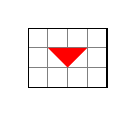
\begin{tikzpicture}[scale=0.25]
    \draw[gray] (-2,2) grid (2,-1); \draw (-2,2) rectangle (2,-1);
    \fill[red,ultra thick] (0,0)--(1,1)--(-1,1)--cycle;
  \end{tikzpicture}
  \\~\\
  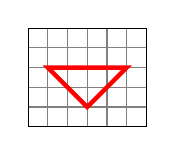
\begin{tikzpicture}[scale=0.25]
    \draw[gray] (-3,4) grid (3,-1); \draw (-3,4) rectangle (3,-1);
    \draw[red, ultra thick] (0,0)--(2,2)--(-2,2)--cycle;
  \end{tikzpicture}
  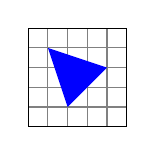
\begin{tikzpicture}[scale=0.25]
    \draw[gray] (-2,4) grid (3,-1); \draw (-2,4) rectangle (3,-1);
    \fill[blue] (0,0)--(2,2)--(-1,3)--cycle;
  \end{tikzpicture}
  \\~\\
  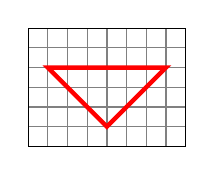
\begin{tikzpicture}[scale=0.25]
    \draw[gray] (-4,5) grid (4,-1); \draw (-4,5) rectangle (4,-1);
    \draw[red, ultra thick] (0,0)--(3,3)--(-3,3)--cycle;
  \end{tikzpicture}
  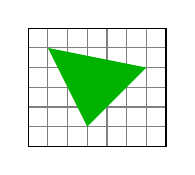
\begin{tikzpicture}[scale=0.25]
    \draw[gray] (-3,5) grid (4,-1); \draw (-3,5) rectangle (4,-1);
    \fill[black!30!green] (0,0)--(3,3)--(-2,4)--cycle;
  \end{tikzpicture}
  \\~\\
  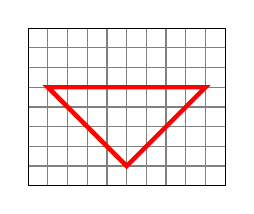
\begin{tikzpicture}[scale=0.25]
    \draw[gray] (-5,7) grid (5,-1); \draw (-5,7) rectangle (5,-1);
    \draw[red, ultra thick] (0,0)--(4,4)--(-4,4)--cycle;
  \end{tikzpicture}
  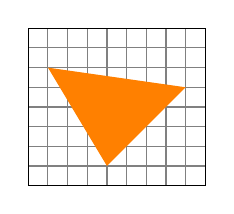
\begin{tikzpicture}[scale=0.25]
    \draw[gray] (-4,7) grid (5,-1); \draw (-4,7) rectangle (5,-1);
    \fill[orange] (0,0)--(4,4)--(-3,5)--cycle;
  \end{tikzpicture}
  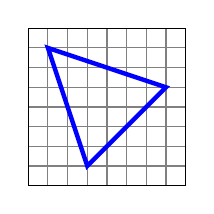
\begin{tikzpicture}[scale=0.25]
    \draw[gray] (-3,7) grid (5,-1); \draw (-3,7) rectangle (5,-1);
    \draw[blue, ultra thick] (0,0)--(4,4)--(-2,6)--cycle;
  \end{tikzpicture}
  \\~\\
  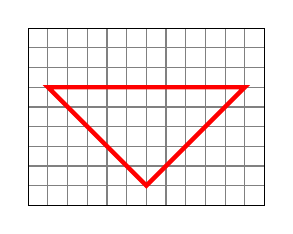
\begin{tikzpicture}[scale=0.25]
    \draw[gray] (-6,8) grid (6,-1); \draw (-6,8) rectangle (6,-1);
    \draw[red, ultra thick] (0,0)--(5,5)--(-5,5)--cycle;
  \end{tikzpicture}
  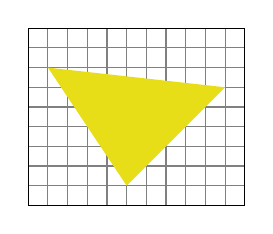
\begin{tikzpicture}[scale=0.25]
    \draw[gray] (-5,8) grid (6,-1); \draw (-5,8) rectangle (6,-1);
    \fill[black!10!yellow] (0,0)--(5,5)--(-4,6)--cycle;
  \end{tikzpicture}
  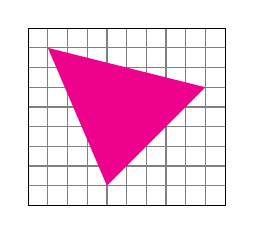
\begin{tikzpicture}[scale=0.25]
    \draw[gray] (-4,8) grid (6,-1); \draw (-4,8) rectangle (6,-1);
    \fill[magenta] (0,0)--(5,5)--(-3,7)--cycle;
  \end{tikzpicture}
  \\~\\
  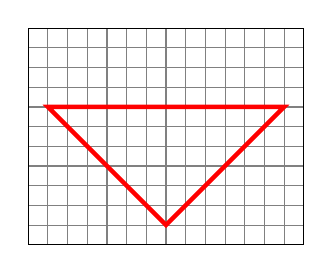
\begin{tikzpicture}[scale=0.25]
    \draw[gray] (-7,10) grid (7,-1); \draw (-7,10) rectangle (7,-1);
    \draw[red, ultra thick] (0,0)--(6,6)--(-6,6)--cycle;
  \end{tikzpicture}
  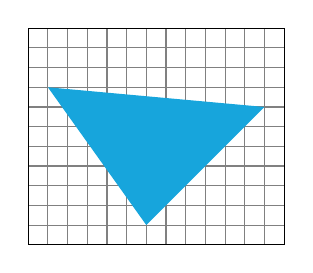
\begin{tikzpicture}[scale=0.25]
    \draw[gray] (-6,10) grid (7,-1); \draw (-6,10) rectangle (7,-1);
    \fill[black!10!cyan] (0,0)--(6,6)--(-5,7)--cycle;
  \end{tikzpicture}
  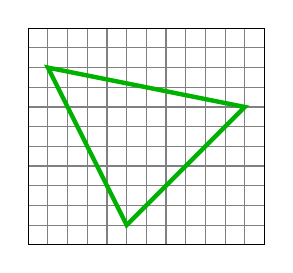
\begin{tikzpicture}[scale=0.25]
    \draw[gray] (-5,10) grid (7,-1); \draw (-5,10) rectangle (7,-1);
    \draw[black!30!green, ultra thick] (0,0)--(6,6)--(-4,8)--cycle;
  \end{tikzpicture}
  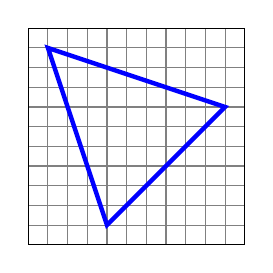
\begin{tikzpicture}[scale=0.25]
    \draw[gray] (-4,10) grid (7,-1); \draw (-4,10) rectangle (7,-1);
    \draw[blue, ultra thick] (0,0)--(6,6)--(-3,9)--cycle;
  \end{tikzpicture}
  \caption{
    An example of $a(1)=1$, $a(2)=1$, $a(3)=1$, $a(4)=1$, $a(5)=2$, and
    $a(6)=1$.
  }
\end{figure}

\begin{question}
  How many triangles of side length $2n$ exist?
  % a(1) = 1
  % a(c) = floor(c/2) - (sum_{d|c} a(d)) % where d are proper divisors of c.
  % a(1)  -> 1                      = 1
  % a(2)  -> 2 - a(1)               = 1
  % a(3)  -> 2 - a(1)               = 1
  % a(4)  -> 3 - a(2) - a(1)        = 1
  % a(5)  -> 3 - a(1)               = 2
  % a(6)  -> 4 - a(1) - a(2) - a(3) = 1
  % a(7)  -> 4 - a(1)               = 3
  % a(8)  -> 5 - a(1) - a(2) - a(4) = 2
  % a(9)  -> 5 - a(1) - a(3)        = 3
  % a(10) -> 6 - a(1) - a(2) - a(5) = 2
\end{question}
\begin{note}
  The answer is probably that $a(1) = 1$ and $a(n) = \lfloor n/2 \rfloor + 1 - \sum_{d|n} a(d)$,
  which appears to be $A023022$.
\end{note}
\begin{related}
  \item What is the related sequence for triangles measured under the $d_\infty$
    metric?
  \item How does this generalize to equilateral $n$-gons? Convex $n$-gons?
  \item How does this generalize to a Taxicab-like metric on a triangular grid?
\end{related}
\begin{references}
  \item \url{http://oeis.org/A023022}
\end{references}
\end{document}
